\documentclass[resume]{subfiles}


\begin{document}
\section{Chaînes de Markov}
Les chaînes de Markov n'ont \textbf{pas de mémoire}. L'état actuel encode la totalité de la chaîne
\paragraph{Chaîne de Markov homogène} : Chaîne pour laquelle la probabilité de transition de l'état $i$ à $j$ est toujours la même, indépendamment du points à laquelle est est arrivée.
\subsection{Représentation graphique}
\begin{figure}[H]
\centering
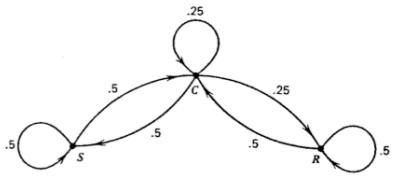
\includegraphics[width=6cm]{img_15.png}
\end{figure}
\subsection{Représentation matricielle}
\begin{figure}[H]
\centering
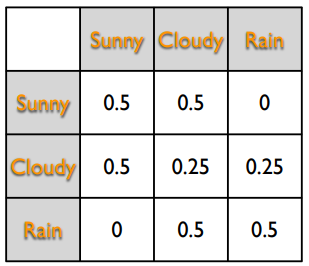
\includegraphics[width=5cm]{img_16.png}
\end{figure}
$$P=\begin{bmatrix}
p_{11} & p_{12} & \cdots & p_{1n}\\
p_{21} & p_{22} & \cdots & p_{2n}\\
\vdots & \vdots & \ddots & \vdots\\
p_{n1} & p_{n2} & \cdots & p_{nn}
\end{bmatrix}$$
La somme de chaque colonne / ligne est $1$
\subsection{Vecteur de probabilité d'état}
$\pi(0)$ est le vecteur de probabilité à l'itération 0 ($1$ à la ligne qui correspond à l'état initial). On calcule la probabilité de chaque état de manière itérative
$$\pi(1)=P^{T}\pi(0)$$
$$\pi(k+1)=P^{T}\pi(k)$$
$$\pi(k)=P^{T^{k}}\pi(0)$$
\subsection{État récurrent}
Si une chaine revient sur un état précédent, c'est un état récurrent
\subsection{État stable}
l'état de stabilité $\pi$ est tel que
$$\pi = P^T\pi$$
$$\lim_{m\to\infty}P^m=\bar{P}$$




\end{document}